%Full Report = Includes Introduction and Conclusion. Re-write experiments, integrate graphs, analysis, and comments to
%make a clean easy to read report. Your report must include carbonless copies of in-lab notes. Type written reports.
\documentclass[10pt,letterpaper,oneside] {article}
\usepackage{graphicx}
\usepackage{amsmath}
\usepackage[normalem]{ulem}
\usepackage[hidelinks]{hyperref}
\usepackage{natbib}
\hypersetup{colorlinks,urlcolor=blue}
%\usepackage[labelformat=empty]{caption}
% hack into hyperref
\makeatletter
\usepackage[margin=1.0in]{geometry}
\newcommand{\tab}[1]{\hspace{.26\textwidth}\rlap{#1}}
%\renewcommand{\labelitemii}{$\cdot$}
\renewcommand{\labelitemiii}{$\diamond$}
\begin{document}
\title{Introductory Experiments and Linear Circuits I}
\author{\quad \\Jung Lin (Doris) Lee [Lab Partner: Leah Tom]\\Prof. William Holzapfel, GSI Thomas Darlington, Thomas Mittiga, John Groh,  \\Victoria Xu, Jonathan Ma, Francisco Monsalve, Xiaofei Zhou}
\maketitle
	\begin{abstract}
	In this lab, we explore ----- BSC 
	\end{abstract}


\section{Introduction}
 
\paragraph{\textbf{1.2}} 

\paragraph{\textbf{1.4}} 
   
 \section{Keithley 2110 Digital Multimeter3 (DMM)}
- uncertainty
The range should be adjusted  suitable range within --- for each measurement , within order of magnitude. \footnote{Too large a range will result in the error ``OVLRD" (overload) and too low will cause ---}
\section{BSC Laboratory Breadboard Box}
\begin{figure}[h!]
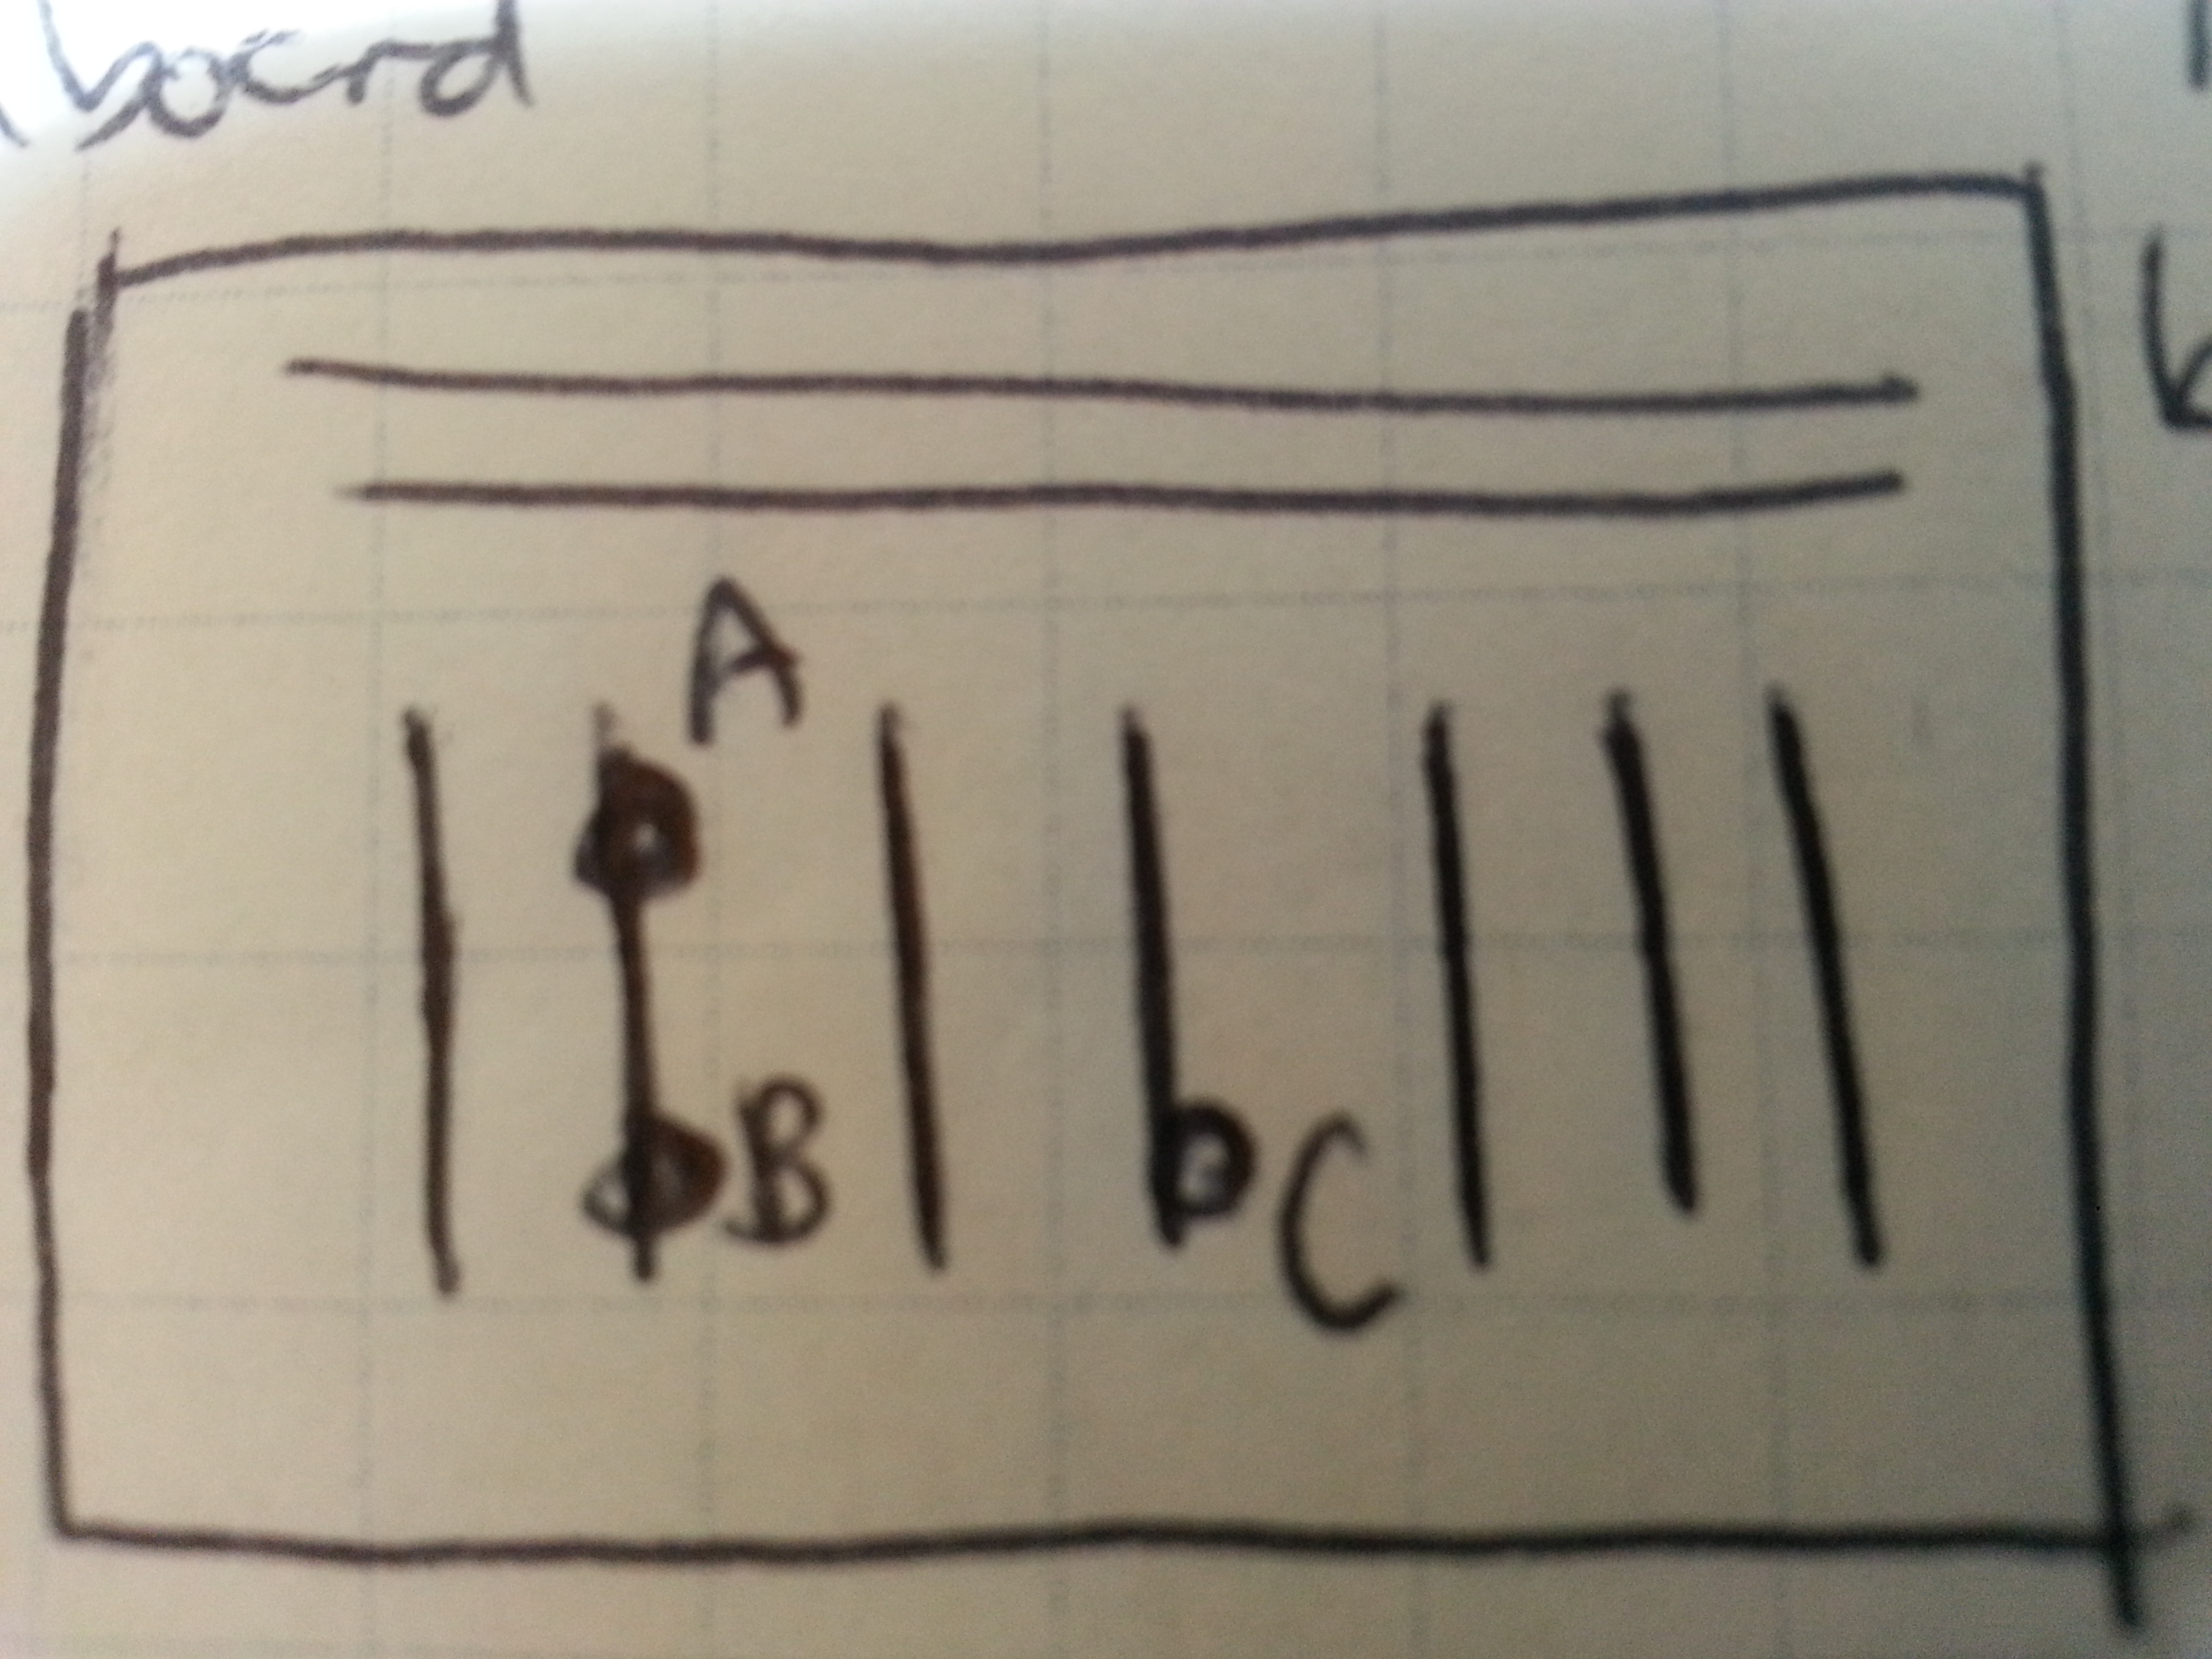
\includegraphics[width=200pt]{figure/d_breadboard}
\caption{We put jumper wires connecting the A and B, B and C separately and measure the resistance across them.}
\label{breadboard}
\end{figure}
\paragraph{\textbf{1.1}}
The breadboard is a device suitable for rapid-protoyping circuits, without long chemical etching process of the PCB.  As shown in Fig.\ref{breadboard} , it is horizontally connected along the longer edge for the two top and bottom buses, which often serves as to input voltage and grounding --. We measured the resistance across A and B as 0.16 $\Omega$ and across B and C as ``overload".  These result make sense because since B and C is not connected, the resistance is almost infinite, and is therefore not registered on the DMM. Likewise, since A and B are connected, there is minimal resistance between them.
\paragraph{\textbf{1.3}} 
The reading between the 12 output and the 5V supply ground fluctuates around 0V. The reason why ----.
\paragraph{\textbf{1.5}} \label{1_5}
Since the resistors are arranged in series as shown in Fig.\ref{voltage_divider}, the current through each resistor should be the same. 
\begin{equation}
I = \frac{V}{R_{eq}}=\frac{V}{R_1+R_2}=\frac{24V}{480\times10^3\Omega
}= 5/0\times10^{-5}A 
\end{equation}
\begin{figure}[h!]
\center
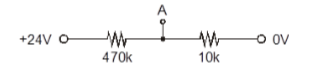
\includegraphics[width=200pt]{figure/d_voltage_divider}
\caption{Voltage divider setup}
\label{voltage_divider}
\end{figure}
\paragraph{\textbf{1.7}} 
a) Depending on the DMM setup, it can act as a voltmeter or ammeter. To meaaure the current through a 10k$\Omega$ resistor, we need to connect the DMM in parlalle with the 10k$\Omega$ resistor as shown in Fig. ---- 
Then, using Ohm's law we can compute the current flowing through the 10k$\Omega$ resistor: 
\begin{equation}
I = \frac{V}{R}=\frac{0.510V}{10k\Omega}=5.1\times 10^-5 A
\label{current}
\end{equation}
which is approximately the same as predicted in \ref{1_5}. Alternatively, we can also connect the multimeter in series with the resistor as shown in Fig. \ref{ammeter}  \footnote{Note that the ---- terminate need to be plugged into the hole that  ---- and --- instead of the --- and ---- as when we do the voltage measurement. The left 2 ---- gives a better accuracy} to measure the current directly, and this yields the same current value as computed in Eq.\ref{current}.
\begin{figure}[h!]
\center
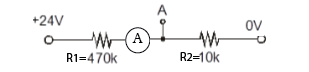
\includegraphics[width=200pt]{figure/ammeter}
\label{ammeter}
\end{figure}
\\
b)  
\section{Digital Oscilloscope}
voltage on the vertical axes and time on the horizontal axes
\subsection{Tune-able Parameters and useful functions}
\begin{itemize}
\item AC/DC Setting : (See Sec.\ref{sec:acdc})
\item Scale: Vertical and horizontal zoom in ; adjust accordingly to --- window that best captures
\item Measurement: useful quantities 
\end{itemize}
\section{Arbitrary Waveform Function Generator}
\section{Frequency and time measurements}
\subsection{AC measurement}\label{sec:acdc}
\section{Thevinin Equivalence}
\begin{figure}[h!]
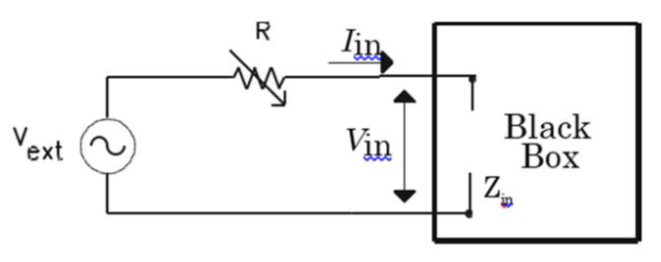
\includegraphics[width=200pt]{figure/d_Z_input}
\label{Z_input}
\end{figure}
\begin{figure}[h!]
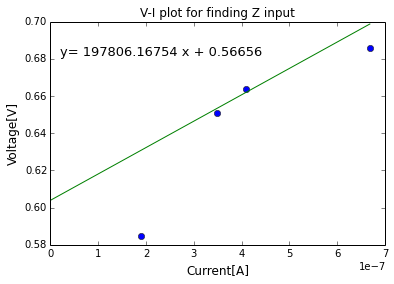
\includegraphics[width=200pt]{figure/Z_input_plot}
\caption{Voltage measurement has uncertainty of 0.001V . }
\label{Z_input_plots}
\end{figure}
\paragraph{\textbf{2.3}}
We treat the oscilloscope as a black box of unknown impedance.  We substituted different resistors in the circuit shown in  Fig.\ref{Z_input}, and measured the input voltage. Using Eq.\ref{I_input} , we can compute the input current as plotted in Fig. \ref{Z_input_plots}
\begin{equation}
I_{in} =\frac{V_{ext}-V{in}}{R}
\label{I_input}
\end{equation}
A linear regression on the data results in a slope of 0.197806 M$\Omega$. Since  $Z_{in}=\frac{V_{in}}{V_{ext}-V_{in}}R =\frac{V_{in}}{I_{in}}$, the value of the slope is equivalent to the  input impedance, which is the same order of magnitude as the input impedance of typical oscilloscope ( $\approx$ 1 M$\Omega$). \cite{tekronix}

%\subsection{2.1.14}
%Given $v = 2/3c$, $\Delta$ d  = 10ft = 30.48m :
%\begin{equation}
%\Delta t = \frac{\Delta d}{v} = \frac{30.48m}{\frac{2}{3}\times 299792458 m/s} = 1.525 ns
%\end{equation}
%By comparing the difference between the signals in Fig. ----- peak-to-peak
 \section{Conclusion}
\section{Acknowledgments}
The author would  like to acknowledge support from the GSI in --- this lab --.  I thank my partner, Leah Tom, for helpful discussion and ----- collaboration that helped this work.
\bibliography{references}
\bibliographystyle{plain}
\end{document}